\chapter{Omisión de palabras}

Anteriormente se especificó que la base de datos de los préstamos serían únicamente palabras de contenido, y a partir de ellas se realizaron los análisis anteriores.  Al trabajar con esta clasificación se están restringiendo a todas las palabras que pueden ser catalogadas como préstamos (algunos artículos o pronombres de un determinado idioma se encuentran en los demás), sin embargo los resultados obtenidos han reflejado contextos históricos en los cuáles explicar los movimientos de las palabras, por lo que las restricciones han ayudado a las deducciones. 

Por el momento ya no se tratara con la misma regularidad a la interpretación histórica de las migraciones, se centrará la siguiente parte en tratar a los prestamos como un conjunto que muestra la propiedad del uso de un idioma en otro, y ver como es afectada esta propiedad si es modificado el conjunto. 

La manera de alterar a los prestamos, se realizará al hacer restricciones en las palabras que conforman el conjunto; como antecedente se tiene el haber eliminado todas las palabras funcionales  y utilizar las de contenido.  Como todos los préstamos son palabras de contenido, las restricciones consistirán en eliminar las palabras que comiencen con ciertas letras.

\hfill\break

El proceso es sencillo y consiste en lo siguiente:
 


\begin{enumerate}
	
	\item Se eligen una pareja de idioma origen $\textit{A}$ e idioma receptor $\textit{B}$. Considerando como verdadero el uso de $\textit{A}$  en $\textit{B}$. 
	
	\item Se escogen de forma aleatoria un conjunto de letras (desde una hasta cuatro), y se eliminan del conjunto de prestamos de $\textit{A}$  en $\textit{B}$ a todas las palabras cuya primer letra sea alguna de las elegidas.  
	
	\item Se designan tres conjuntos:
	
		\begin{itemize}
			\item \textbf{Conjunto original:} Conformado por todos los prestamos de $\textit{A}$  en $\textit{B}$.
			\item \textbf{Conjunto reducido:} Conjunto original menos las palabras eliminadas. 
			\item \textbf{Conjunto residuo:} Conformado por las palabras eliminadas del conjunto original. 
		\end{itemize}
	
	\item En cada conjunto se empleo la ecuación \ref{ec.fuso} para obtener el uso de $\textit{A}$ en $\textit{B}$  con los elementos de cada conjunto. 
	
\end{enumerate}


Por la cantidad de elementos que contiene el conjunto residuo, el uso entre idiomas utilizando este conjunto es despreciable con los valores obtenidos para el conjunto original y el reducido.  Cabe decir que entre mas letras se escojan para reducir el conjunto, el residuo tendrá cada vez más elementos siendo en algun momento comparable al original.  Por ello se decidió que el máximo de restricciones fuese de cuatro letras. 

La forma de las graficas del uso del conjunto original es el mismo que se presentó en el capitulo anterior, sólo que ahora se graficaran en color negro sin importar que combinación de idiomas se este tratando.  Para el conjunto reducido cada valor de uso se marco en color rojo.  En cada grafica se especifica que letras se usaron para reducir al conjunto.


\subsubsection*{Inglés}

\begin{figure}[h!]
	\centering
	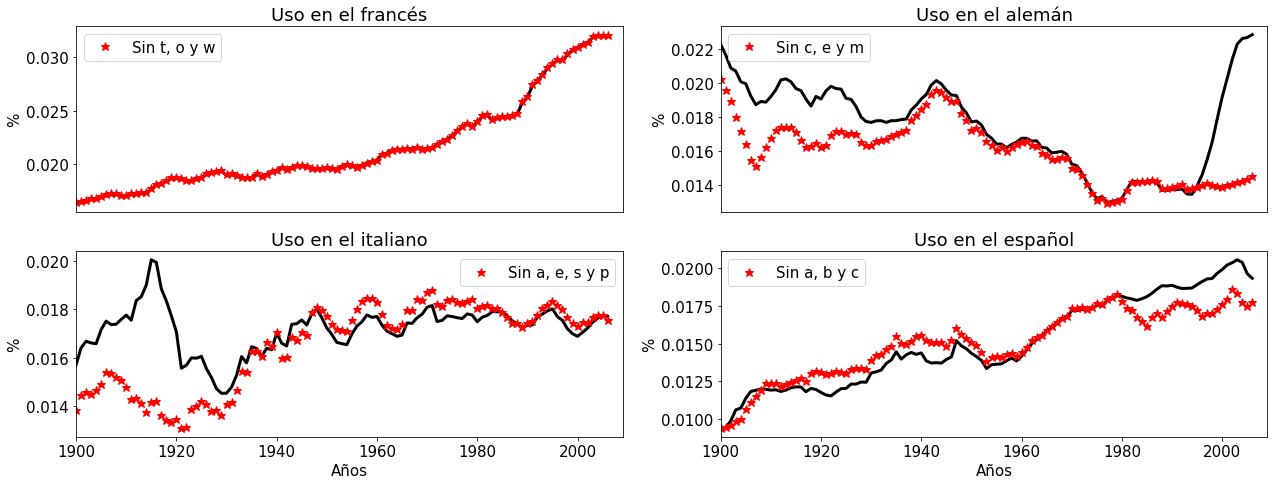
\includegraphics[width=14.5cm, height=7cm]{Cap_5/OM_EN.png}
	\label{fig.OM_EN}
	\caption{Omisiones del inglés en los demás}
\end{figure}

\newpage
\subsubsection*{Francés}

\begin{figure}[h!]
	\centering
	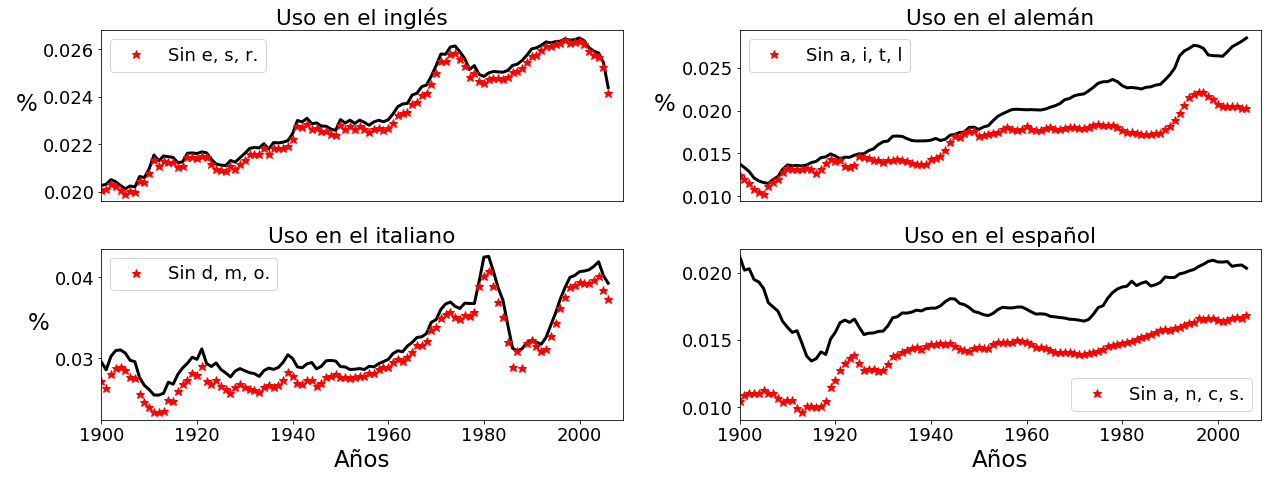
\includegraphics[width=14.5cm, height=7cm]{Cap_5/OM_FR.png}
	\label{fig.OM_FR}
	\caption{Omisiones del francés en los demás}
\end{figure}



\subsubsection*{Alemán}

\begin{figure}[h!]
	\centering
	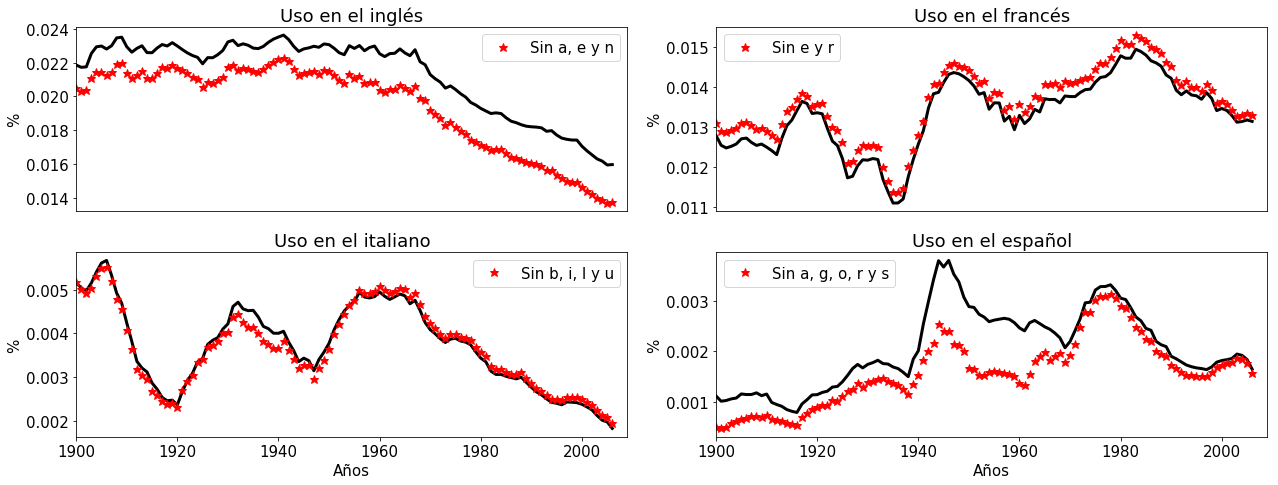
\includegraphics[width=14.5cm, height=7cm]{Cap_5/OM_GE.png}
	\label{fig.OM_GE}
	\caption{Omisiones del alemán en los demás}
\end{figure}

\newpage
\subsubsection*{Italiano}

\begin{figure}[h!]
	\centering
	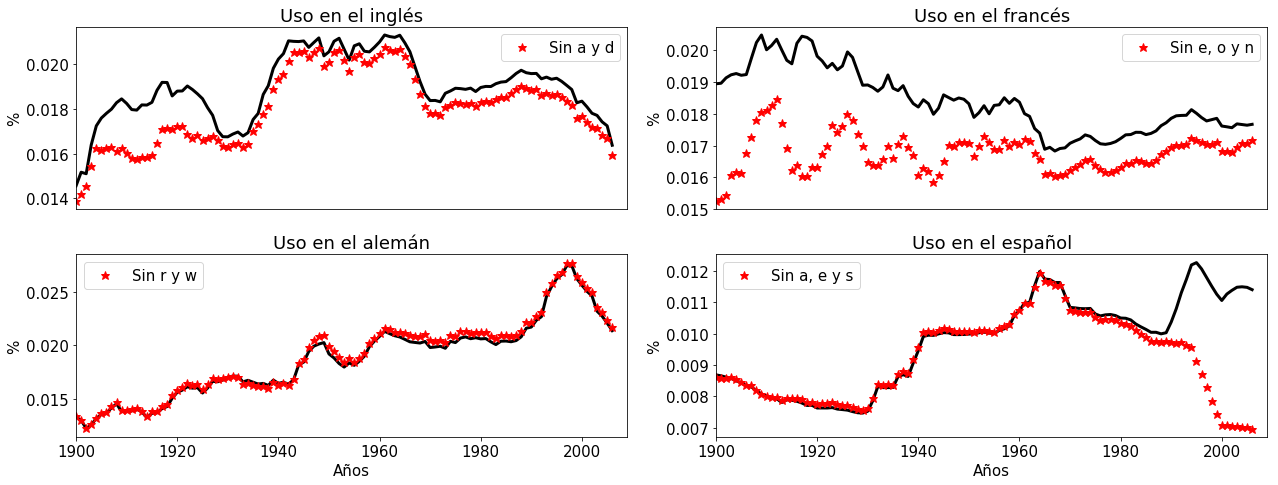
\includegraphics[width=14.5cm, height=7cm]{Cap_5/OM_IT.png}
	\label{fig.OM_IT}
	\caption{Omisiones del italiano en los demás}
\end{figure}


\subsubsection*{Español}

\begin{figure}[h!]
	\centering
	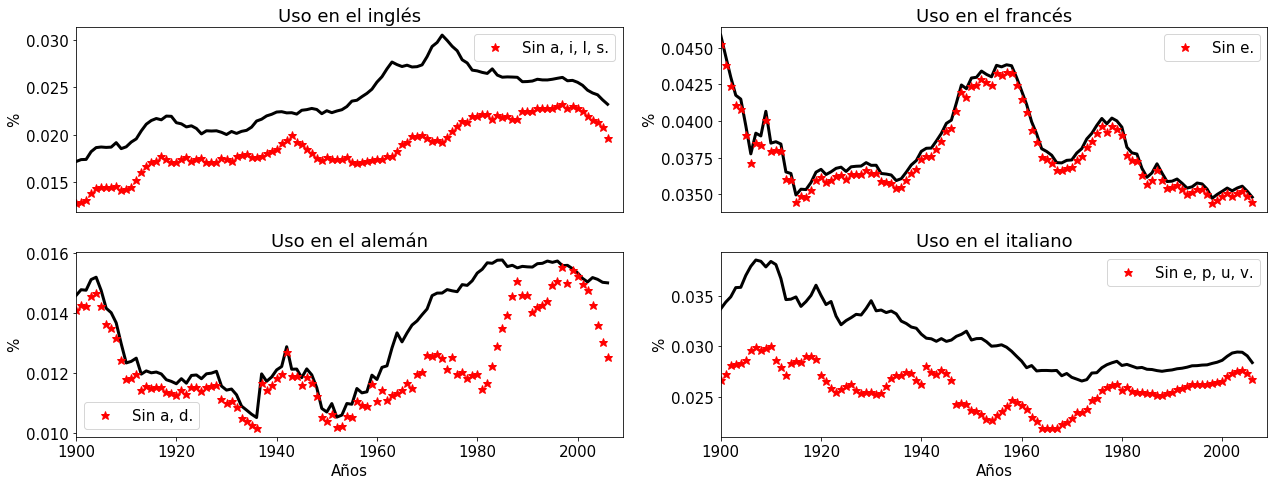
\includegraphics[width=14cm, height=7cm]{Cap_5/OM_SP.png}
	\label{fig.OM_SP}
	\caption{Omisiones del español en los demás}
\end{figure}
